% Options for packages loaded elsewhere
\PassOptionsToPackage{unicode}{hyperref}
\PassOptionsToPackage{hyphens}{url}
%
\documentclass[
]{book}
\usepackage{amsmath,amssymb}
\usepackage{iftex}
\ifPDFTeX
  \usepackage[T1]{fontenc}
  \usepackage[utf8]{inputenc}
  \usepackage{textcomp} % provide euro and other symbols
\else % if luatex or xetex
  \usepackage{unicode-math} % this also loads fontspec
  \defaultfontfeatures{Scale=MatchLowercase}
  \defaultfontfeatures[\rmfamily]{Ligatures=TeX,Scale=1}
\fi
\usepackage{lmodern}
\ifPDFTeX\else
  % xetex/luatex font selection
\fi
% Use upquote if available, for straight quotes in verbatim environments
\IfFileExists{upquote.sty}{\usepackage{upquote}}{}
\IfFileExists{microtype.sty}{% use microtype if available
  \usepackage[]{microtype}
  \UseMicrotypeSet[protrusion]{basicmath} % disable protrusion for tt fonts
}{}
\makeatletter
\@ifundefined{KOMAClassName}{% if non-KOMA class
  \IfFileExists{parskip.sty}{%
    \usepackage{parskip}
  }{% else
    \setlength{\parindent}{0pt}
    \setlength{\parskip}{6pt plus 2pt minus 1pt}}
}{% if KOMA class
  \KOMAoptions{parskip=half}}
\makeatother
\usepackage{xcolor}
\usepackage{color}
\usepackage{fancyvrb}
\newcommand{\VerbBar}{|}
\newcommand{\VERB}{\Verb[commandchars=\\\{\}]}
\DefineVerbatimEnvironment{Highlighting}{Verbatim}{commandchars=\\\{\}}
% Add ',fontsize=\small' for more characters per line
\usepackage{framed}
\definecolor{shadecolor}{RGB}{248,248,248}
\newenvironment{Shaded}{\begin{snugshade}}{\end{snugshade}}
\newcommand{\AlertTok}[1]{\textcolor[rgb]{0.94,0.16,0.16}{#1}}
\newcommand{\AnnotationTok}[1]{\textcolor[rgb]{0.56,0.35,0.01}{\textbf{\textit{#1}}}}
\newcommand{\AttributeTok}[1]{\textcolor[rgb]{0.13,0.29,0.53}{#1}}
\newcommand{\BaseNTok}[1]{\textcolor[rgb]{0.00,0.00,0.81}{#1}}
\newcommand{\BuiltInTok}[1]{#1}
\newcommand{\CharTok}[1]{\textcolor[rgb]{0.31,0.60,0.02}{#1}}
\newcommand{\CommentTok}[1]{\textcolor[rgb]{0.56,0.35,0.01}{\textit{#1}}}
\newcommand{\CommentVarTok}[1]{\textcolor[rgb]{0.56,0.35,0.01}{\textbf{\textit{#1}}}}
\newcommand{\ConstantTok}[1]{\textcolor[rgb]{0.56,0.35,0.01}{#1}}
\newcommand{\ControlFlowTok}[1]{\textcolor[rgb]{0.13,0.29,0.53}{\textbf{#1}}}
\newcommand{\DataTypeTok}[1]{\textcolor[rgb]{0.13,0.29,0.53}{#1}}
\newcommand{\DecValTok}[1]{\textcolor[rgb]{0.00,0.00,0.81}{#1}}
\newcommand{\DocumentationTok}[1]{\textcolor[rgb]{0.56,0.35,0.01}{\textbf{\textit{#1}}}}
\newcommand{\ErrorTok}[1]{\textcolor[rgb]{0.64,0.00,0.00}{\textbf{#1}}}
\newcommand{\ExtensionTok}[1]{#1}
\newcommand{\FloatTok}[1]{\textcolor[rgb]{0.00,0.00,0.81}{#1}}
\newcommand{\FunctionTok}[1]{\textcolor[rgb]{0.13,0.29,0.53}{\textbf{#1}}}
\newcommand{\ImportTok}[1]{#1}
\newcommand{\InformationTok}[1]{\textcolor[rgb]{0.56,0.35,0.01}{\textbf{\textit{#1}}}}
\newcommand{\KeywordTok}[1]{\textcolor[rgb]{0.13,0.29,0.53}{\textbf{#1}}}
\newcommand{\NormalTok}[1]{#1}
\newcommand{\OperatorTok}[1]{\textcolor[rgb]{0.81,0.36,0.00}{\textbf{#1}}}
\newcommand{\OtherTok}[1]{\textcolor[rgb]{0.56,0.35,0.01}{#1}}
\newcommand{\PreprocessorTok}[1]{\textcolor[rgb]{0.56,0.35,0.01}{\textit{#1}}}
\newcommand{\RegionMarkerTok}[1]{#1}
\newcommand{\SpecialCharTok}[1]{\textcolor[rgb]{0.81,0.36,0.00}{\textbf{#1}}}
\newcommand{\SpecialStringTok}[1]{\textcolor[rgb]{0.31,0.60,0.02}{#1}}
\newcommand{\StringTok}[1]{\textcolor[rgb]{0.31,0.60,0.02}{#1}}
\newcommand{\VariableTok}[1]{\textcolor[rgb]{0.00,0.00,0.00}{#1}}
\newcommand{\VerbatimStringTok}[1]{\textcolor[rgb]{0.31,0.60,0.02}{#1}}
\newcommand{\WarningTok}[1]{\textcolor[rgb]{0.56,0.35,0.01}{\textbf{\textit{#1}}}}
\usepackage{longtable,booktabs,array}
\usepackage{calc} % for calculating minipage widths
% Correct order of tables after \paragraph or \subparagraph
\usepackage{etoolbox}
\makeatletter
\patchcmd\longtable{\par}{\if@noskipsec\mbox{}\fi\par}{}{}
\makeatother
% Allow footnotes in longtable head/foot
\IfFileExists{footnotehyper.sty}{\usepackage{footnotehyper}}{\usepackage{footnote}}
\makesavenoteenv{longtable}
\usepackage{graphicx}
\makeatletter
\def\maxwidth{\ifdim\Gin@nat@width>\linewidth\linewidth\else\Gin@nat@width\fi}
\def\maxheight{\ifdim\Gin@nat@height>\textheight\textheight\else\Gin@nat@height\fi}
\makeatother
% Scale images if necessary, so that they will not overflow the page
% margins by default, and it is still possible to overwrite the defaults
% using explicit options in \includegraphics[width, height, ...]{}
\setkeys{Gin}{width=\maxwidth,height=\maxheight,keepaspectratio}
% Set default figure placement to htbp
\makeatletter
\def\fps@figure{htbp}
\makeatother
\setlength{\emergencystretch}{3em} % prevent overfull lines
\providecommand{\tightlist}{%
  \setlength{\itemsep}{0pt}\setlength{\parskip}{0pt}}
\setcounter{secnumdepth}{5}
\usepackage{booktabs}
\usepackage{amsthm}
\makeatletter
\def\thm@space@setup{%
  \thm@preskip=8pt plus 2pt minus 4pt
  \thm@postskip=\thm@preskip
}
\makeatother
\ifLuaTeX
  \usepackage{selnolig}  % disable illegal ligatures
\fi
\IfFileExists{bookmark.sty}{\usepackage{bookmark}}{\usepackage{hyperref}}
\IfFileExists{xurl.sty}{\usepackage{xurl}}{} % add URL line breaks if available
\urlstyle{same}
\hypersetup{
  pdftitle={Nusses kogebog},
  pdfauthor={Christian Knudsen},
  hidelinks,
  pdfcreator={LaTeX via pandoc}}

\title{Nusses kogebog}
\author{Christian Knudsen}
\date{2025-01-19}

\begin{document}
\maketitle

{
\setcounter{tocdepth}{1}
\tableofcontents
}
\hypertarget{welcome}{%
\chapter{Welcome}\label{welcome}}

Hej. Dette er det køkken jeg drømmer om. Indtil da:
Dette er min kogebog. Nusses samling af opskrifter - dimensioneret efter os to derhjemme.

\includegraphics{images/DALL·E-dieselpunk.png}

\hypertarget{gris}{%
\chapter{Gris}\label{gris}}

\hypertarget{bacon-medisterpuxf8lse-i-airfryer}{%
\section{Bacon medisterpølse i airfryer}\label{bacon-medisterpuxf8lse-i-airfryer}}

Medisterpølse vikles ind i bacon.
30 minutter i airfryer ved 180 grader.

\hypertarget{retter-med-kylling}{%
\chapter{Retter med kylling}\label{retter-med-kylling}}

\hypertarget{chicken-piccata}{%
\section{Chicken Piccata}\label{chicken-piccata}}

Fra VEEP

Boneless, skinless chicken breasts
Salt \& pepper
Flour for dredging
Butter
Olive oil
Chicken stock
Shallots
Garlic
Lemons, they brighten everything, including our Lemon Butter Chicken.
Capers

Slice the chicken breasts horizontally---you'll need a sharp knife for this, obviously! The reason you cut the chicken breast into thin pieces is so that they can cook evenly during the pan-frying process. Thin pieces of chicken mean that when the outside is crispy and perfectly brown, the chicken will be cooked through. Magic!
Dredge! Season the chicken breast pieces, and then give them a nice coating of flour. For whatever reason, kids really love to help out with this step. If they're old enough to know to be careful with raw poultry, go ahead and outsource this step to them!
Fry! Fry the chicken cutlets in a combination of olive oil and butter. The oil helps prevent the butter from burning, plus, we love the flavor of both!

Our piccata sauce is simply a pan sauce, which means that we use the good crispy, chicken-tinged buttery bits that are left in the skillet after frying the chicken cutlets to make a sauce. Here's how to make this lemony piccata sauce:

Sauté shallots and garlic in the pan drippings---i.e.~the leftover oil and butter.
Add stock! This is your chance to scrape up those tasty brown bits from the bottom of the pan.
Stir in more butter, plus the requisite capers and lemon juice.
Season with a little salt and pepper.
That's it! You made a pan sauce!

\hypertarget{kyllingetuxe6rte}{%
\section{Kyllingetærte}\label{kyllingetuxe6rte}}

\begin{itemize}
\tightlist
\item
  1 kylling
\item
  2 løg
\item
  5 fed hvidløg
\item
  3 porrer (to rækker)
\item
  4 gulerødder
\item
  4 stilke bladselleri, som vi udelader fordi Kristian ikke er fan af selleri.
\item
  1 pastinak eller persillerod. Stor.
\item
  1/4 kg champignons.
\item
  evt en håndfuld tørrede svampe. Ikke morkler eller den slags. Karl johan eksempelvis.
\item
  Timian
\item
  Laurbærblade 4 stk
\item
  ½ liter kraftig hønsefond
\item
  2 spsk mel - toppet
\item
  1 glas hvidvin (2½ dl)
\item
  2 dl fløde
\item
  Smør
\item
  Olivenolie
\item
  Butterdej
\end{itemize}

Fjern rygbenet fra kyllingen med en fjerkræsaks. skær brystbenet frit og ud.
krydr med salt og peber invendigt, og læg dyret på en rist med kødsiden opad.
Smør olivenolie på skindet og drys med sat. Bag den i ovnen ved 200 grad i
45 minutter. Det går fint i en airfryer.
Ryg og brystben simrer i onden under låg i en halv times tid så vi får den
smag med. Fisk ben op og tilsæt de tørrede svampe til fonden. Lad dem trække
en 20 minutters tid.
Hak løg - ikke for fint. Hak hvidløg - noget finere. Skær rodfrugterne, porrene
og sellerien (hvis du tager den med) i mundrette stykker. Rens svampene og
halver eller kvart dem.
Olie og smør i en stegegryde - når det er bruset af, først løg, lidt senere
hvidløg, og steg til de falder sammen, de skal ikke være helt karameliserede.
grøntsager og svampe tilsættes, sammen med timian og laurbærbladene. Steg det hele
til de tager en smule farve og rodfrugterner er en smule møre. Drys mel over
og bag af. Tilsæt fond og hvidvin lidt af gangen og kog til det tykner.
Tilsæt fløde og lad det simre yderligere et par minutter. Der kan jævnes lidt
mere med maizena. Det skal være ret tykt.

Når dyret er færdig i ovnen tages det ud og køler nok af til at man kan arbejde
med det. Evt. sprødt skind tages af og skæres i små stykker.
Al snask fra bradepanden skrabes over i gryden.
Pil kødet fra dyret, og sær i mindre tern. Kom det i stuvningen og smag til med
salt og peber. Fisk laurbærblade og timianstilke (hvis du brugte frisk timian)
op. Smid også kyllingeskindet i.

Kom stuvningen i dyb tærteform eller lignede og lad det køle af.
Rul butterdej ud (hvis ikke den kommmer i plade). Pensl kanten på formen med æg
og læg butterdej på som låg. Pensl låget med æg, og skær et snit i midten af
låget, så damp kan slippe ud. Bag i ca 35 minutter ved 200 grader. Lad
den hvile ti minutter inden servering.

\hypertarget{hverdagskylling-med-kremede-svampe}{%
\section{Hverdagskylling med kremede svampe}\label{hverdagskylling-med-kremede-svampe}}

Fra food52

\begin{itemize}
\tightlist
\item
  ½ kg svampe
\item
  4 spsk smør
\item
  ½ kg kyllingebryster - Oprindeligt var det 1 kg
\item
  2½ dl piskefløde (eller madlavningsfløde)
\item
  2 spsk dijon sennep
\item
  finthakket purløg
\end{itemize}

Rens svampene, skær halvdelen i skiver, og resten i kvarter.

\begin{itemize}
\tightlist
\item
  Smelt 2 spsk smør,
\item
  tilføj svampene, steg dem 10-15 minutter, til
  de begynder at karamelisere.
\item
  Halver kyllingebrysterne på langs,
  og bank dem med kødhammeren, ca 1/4 tomme så - 40 millimeter?
\item
  dub dem af, og krydr med salt og peber.
\item
  Giv svampene lidt salt og peber, deglacer med 1/3 cup vand.
\item
  Smelt resten af smørret, steg kyllingerne. Smid gerne en
  bøfpresse ovenpå dem.
\item
  Bland fløde og sennep. Rør dem i svampene, og kog under omrøring
  til den tykner. Smag til med salt, peber og sennep.
\item
  Saml - kylling overhældes med svamep. Vi serverer med ris.
\end{itemize}

\hypertarget{onepot-chicken-rice}{%
\section{Onepot chicken \& rice}\label{onepot-chicken-rice}}

Fra noma

\begin{itemize}
\item
  60 g olie
\item
  4 kyllige lår uden ben, med skind
\item
  salt
\item
  140 gram løg finthakket
\item
  3 fed hvidløg smadret
\item
  15 g tomatpasta
\item
  60 g hvid miso
\item
  15 g røget paprika
\item
  80 g røget svampe garum
\item
  600 g grøntsagsbouillon
\item
  10 g salt
\item
  200 g ris
\item
  10 g persille
\item
  200 g mayonaise
\item
  1 fed hvidløg - revet.
\end{itemize}

Olie varmes op i sautepanden ved middel varme. Krydr kyllingerne med generøse
mængder salt. Når olien simrer, brunes kyllingen på skindsiden (men kun skindsiden),
til den er mørkebrun og sprød. Det skal tage ca. 4 minutter.
Fjern kyllingerne fra panden. Skru ned til lav varme.
tilsæt løg og hvidløg. Steg til løgene er klare.
rør tomatpastaen i og steg ca. 5 minutter til tingene er rustent brune.
Tilsæt bouillon, salt, røget svampe garum, parpirka og miso. Øg temperatren til høj. Rør for at
blande.

Når væsken koger, tilsæt risene og rør så de er jævnt fordelt. Her fra skal risene ikke røres!

Skru ned for varmen, og lad den simre. tilføj kyllingerne til gryden, med den rå side ned. (så ved stegningen
er det kun på skindsiden at den skal steges!) Når duften af brændte ris kan mærkes - efter ca. 20-25 minutter
er vi ca. færdige. tag af varmen, og lad hivle i 5 minutter. pynt med hakket persille.

Bland mayo med hvidløg og bland godt.

Server portioner af ris på tallerken - husk at få det sprøde let brændte lag med. Kylling på toppen.
Top yderligere med hvidløgsmayo.

\hypertarget{pollo-orzo}{%
\section{Pollo orzo}\label{pollo-orzo}}

One pot. Og relativt hurtig.

\begin{figure}
\centering
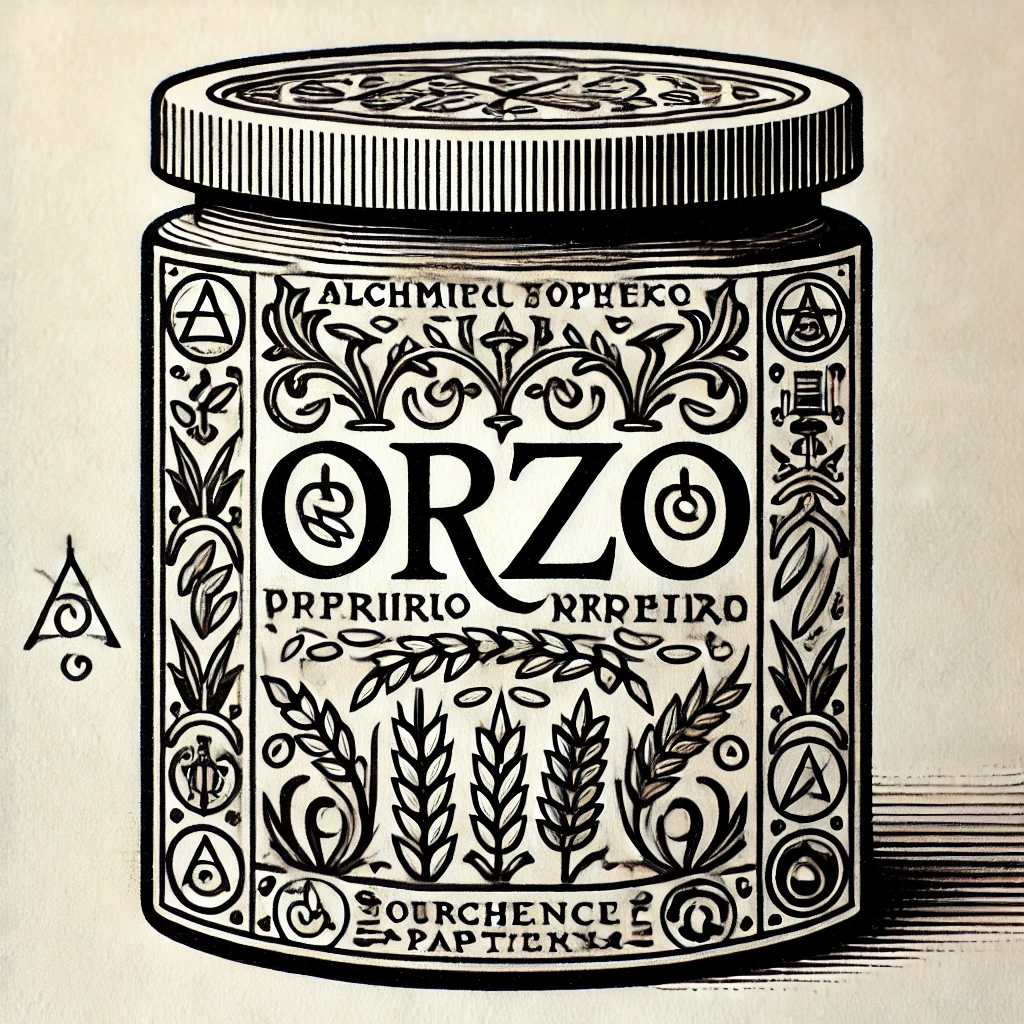
\includegraphics{images/orzo.png}
\caption{orzo}
\end{figure}

Orzo er de der små rislignende pastating.

\begin{itemize}
\tightlist
\item
  Kyllingestykker. Helst med ben. En samling lår er fint.
\item
  3 fed hvidløg
\item
  2 tsk salt
\item
  peber
\item
  1½ liter vand
\item
  \textasciitilde½ liter kyllingefond.
\item
  En dåse hakkede tomater
\item
  1 løg eller to hvis det er et lille løg
\item
  340 gram orzo pasta
\item
  persille
\end{itemize}

Brun killingerne i olie/smør/andefedt/margarine
ca. 5 minutter på hver side.

Tag killingerne op, og brun pastaen let i fedtstoffet.

Tilsæt finthakket løg og klar løgene. Smid finthakket hvidløg i til sidst.

Læg killingerne tilbage i panden.

Hæld fond og tomater over.

Låg på, og lad simre 10-15 minutter, afhængig af orzo type og killing.
Pastaen skal være al dente, killingen skal være gennemstegt/kogt.

Tag gryden af varmen, og lad den hvile i 5 minutter. Orzoen skal gerne absorbere
stort set al væden. Hvis det skal være ekstra festligt, så hæld persille over.

\hypertarget{ko}{%
\chapter{Ko}\label{ko}}

Ko-opskrifter.

\hypertarget{stifatho}{%
\section{Stifatho}\label{stifatho}}

Det har sikkert været med ged eller lam snarere end ko. Men her i huset laves det med ko.
800 g oksetykkam eller lignedne
15 hele løg (lidt afhængig af deres størrelse)
4 fed hvidløg
5 laurbærblade
2 spsk tomatpure
4 dl rødvin
½ kalve eller okse boullion
olivenolie, salt og peber

Puds kødet af og skær det i store tern - 2-4 cm på hver led.
Steg det afpudsede af i en separat gryde, og hæld bouillion over - lad det
simre.
Kødet brunes godt af i stegegryden, gerne af nogle omgange.
Pil løgene og smid dem i gyrden.
Pil hvidløgene og mos dem. De skal også i gryden.
Laurbærbladene kommer også i, og så lader vi det hele få varmen i gryden,
før vi steger tomatpureren af, og hælder rødvin på.
Sigt boullionen, og hæld den i gryden også. Salt og peber skal også i nu.

Skum af, lad simpre i 1½ til to timer (ikke meget længere, så bliver kødet
tørt). Giv gerne løgene nogle tæsk undervejs, og jævn evt. til sidst.

Smag til med salt, peber og rødvin, hvis der er mere tilbage. Server med mos eller
ris.

\hypertarget{lam}{%
\chapter{Lam}\label{lam}}

\hypertarget{lammekuxf8lle}{%
\section{Lammekølle}\label{lammekuxf8lle}}

Vi spiser ikke meget lam. Men til påske skal det være. Opskriften er oprindeligt fundet i Weekendavisen, men justeret undervejs -- så jeg kan dårligt huske hvordan den oprindeligt var.

\begin{itemize}
\tightlist
\item
  1 udbenet lammekølle
\item
  200 g gedeost
\item
  3 fed hvidløg
\item
  2 kviste rosmarin
\item
  20 tørrede abrikoser
\item
  Kartofler -- et par kilo
\item
  En halv liter grøntsagsbouillon
\item
  Salt og peber
\end{itemize}

Rosmarin -- hakket, hvidløg -- hakkede og abrikoserne -- hakkede, blandes med osten.

Lammekøllen stoppes med mixet. Der er ikke plads til det hele -- no worries.

Køllen snøres med bomuldstråd.

Kartoflerne skrælles eller skrubbes, skæres i både og fordeles i en bradepande.

Resten af oste-blandingen fordeles blandt dem. Køllen placeres på en rist over kartoflerne, og hele herligheden får ca. 1½ time i ovnen ved 175 grader.

Kernetemperaturen (i kødet -- ikke i fyldet!) skal lande på ca. 60 grader. Rør gerne rundt i kartoflerne undervejs.

Bønner eller bønnesalat går godt hertil -- det knækker lige den fede smag fra lammet og osten.

\hypertarget{vildt}{%
\chapter{Vildt}\label{vildt}}

\hypertarget{kanin}{%
\section{Kanin}\label{kanin}}

\hypertarget{forloren-gedegryde.}{%
\subsection{Forloren gedegryde.}\label{forloren-gedegryde.}}

Nej, der er ikke ged i. Men når der er improviseret i køkkenet, er spørgsmålet
ofte: ``Hvad hedder det?''. Det aner jeg ikke, jeg har jo improviseret.
Modspørgsmålet er derfor: ``Hvad har du lyst til at kalde det?''.

Svaret denne gang var ``Forloren gedegryde''. Og det er jo rigtig nok. Der er ikke
ægte ged i.

\begin{figure}
\centering
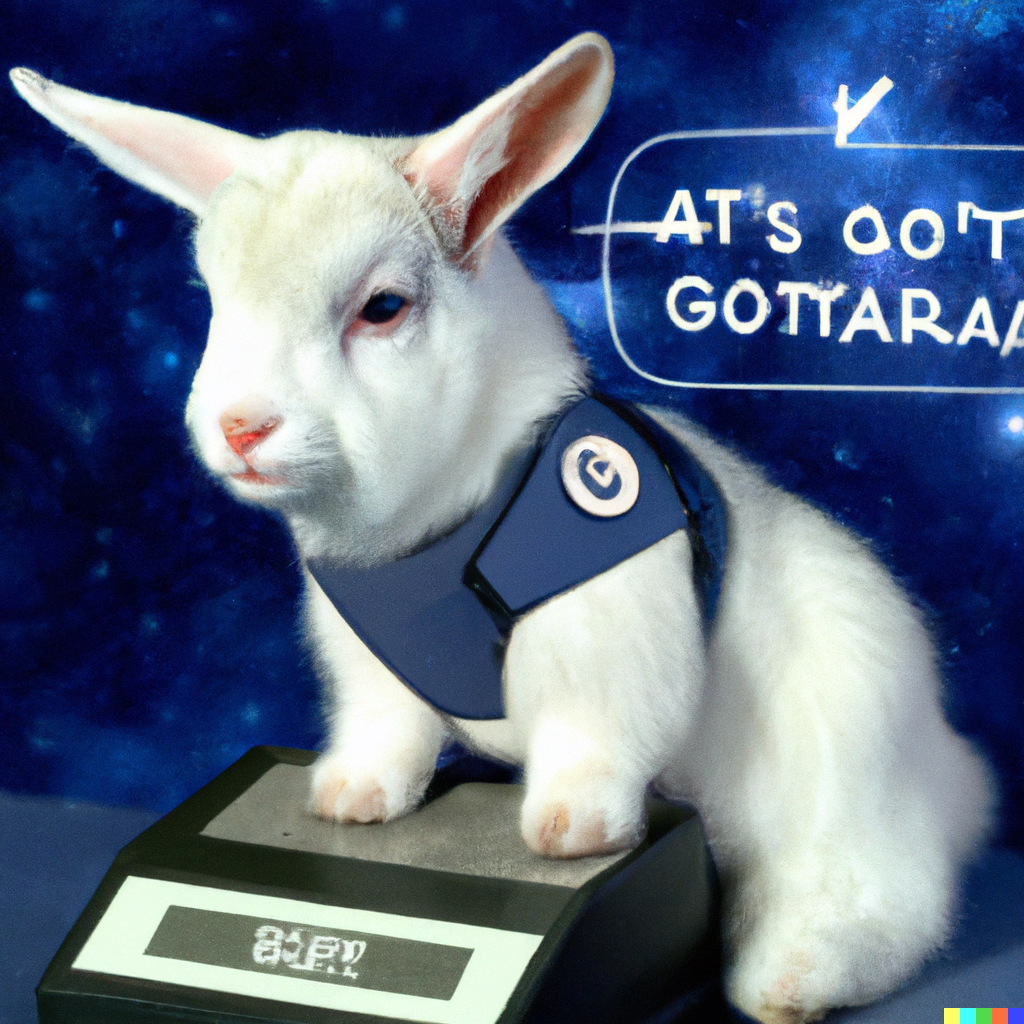
\includegraphics{images/DALL-E-notagoat.png}
\caption{Not a goat}
\end{figure}

\begin{itemize}
\tightlist
\item
  ½ kanin
\item
  1 spsk sennepspulver
\item
  1 finthakket løg
\item
  4 finthakkede hvidløg
\item
  1 æble (skrællet og i mindre stykker)
\item
  ½ rulle gedeost
\item
  2½ dl piskefløde
\item
  ½ liter kyllingefond/mælk
\item
  Lidt sherry
\item
  Smør og mel
\item
  Salt, peber
\end{itemize}

Kaninen gnubbes med salt, peber og en spsk sennepspulver, og hygger sig i køleskabet en 5-6 timer.
Kaninus brunes i stegegryden, og tages op.
Løgene klares, og hvidløg og æble tilsættes, og får lidt varme.
Gryden koges af med en sjat sherry, og fløde, kyllingefond og/eller mælk tilsættes.
Jeg gav den 2½ dl fløde, der var ikke så meget kyllingefond tilbage i skabet, så der blev suppleret op med skummetmælk, til det passede.
En ½ rulle gedeost var til overs fra produktionen af nytårssnacks. Den blev skrællet og dumpet i sovsen også. Kog sovsen igennem til æblerne er gået i opløsning.

Lad Ninka Ninus vende tilbage til gryden, og lad det simre i ca. 20 minutter.
Sovsen jævnes med en melbolle, og smages til med salt, peber og lidt mere sennepspulver.

Jeg serverede den med ris og ærter. Og der blev spist op.

\hypertarget{pasta}{%
\chapter{Pasta}\label{pasta}}

\hypertarget{peberpasta}{%
\section{Peberpasta}\label{peberpasta}}

En Caico e pepe variant

\begin{itemize}
\tightlist
\item
  320 gram pasta
\item
  4 spsk smør (eller oliven olie)
\item
  2 1/4 spsk peber - gerne Triple Lemon Pepper fra Mill \& Mortar
\item
  2½ dl revet parmasan
\item
  hakket persille eller basilikum
\end{itemize}

Kog pastaen til den der er al dente. Dræn, gem kogevand.

Rør pasta sammen med smør i pande eller stor gryde. Tilsæt peber og 2-3 dl
kogevand. Rør mere rundt under god varme.

Tag af kogepladen og tilsæt os. Andret med basilikum eller persille.

Server med stegt kylling, godt brød eller lignende.

\hypertarget{misopasta}{%
\section{Misopasta}\label{misopasta}}

\begin{itemize}
\tightlist
\item
  310 gram pasta - linguine eller bucatini
\item
  6 spsk smør
\item
  3 spsk miso (sådan en vejer 18 gram)
\item
  100 gram revet parmasan
\end{itemize}

Bring vand i kog, og kog pastaen.

Imens samler vi smør og miso i en gryde eller lignende - jeg
bruger min sauterpande. Der røres ret grundigt rundt.
Tilsæt den næsten færdige pasta og 2½ dl eller så kogevand
fra pastaen. Samt parmasanen. Rør aggresivt, indtil
osten er smeltet og sovsen danner en emulsion.

Bum. Server evt noget kylling i skiver, en grøntsag eller noget.

\hypertarget{mac-n-peas}{%
\section{Mac n Peas}\label{mac-n-peas}}

\begin{itemize}
\tightlist
\item
  600 g frostærter
\item
  310 g makaroni
\item
  50 g smør
\item
  3 fed hvidløg
\item
  60 g parmasan
\end{itemize}

Kog ærter og makeroni
Hak hvidløg fint, og lun i smørret på sauterpanden
Overfør de fleste af ærterne til panden, og stavblend sammen med parmasanen (og salt og peber)
De resterende hele ærter, evt også lidt kogevand, samt makeroni røres sammen med ærtemosen i panden.

Server et par af Faktas (nu 365s) flutes til.

\hypertarget{pasta-al-dante}{%
\section{Pasta al Dante}\label{pasta-al-dante}}

Dante skrev i følge overleveringen sine digte på en plads med udsigtover byggepladsen hvor Duomoen blev bygget. I følge rygterne havde han en overmenneskelig hukommelse.
En forbipasserende skulle have spurgt ham hvad der var bedst at spise. Og han svarede prompte ``æg''. Den samme forbipasserende fandt hm et år senere siddende samme sted, og spurgte ``Med hvad''. Hvortil Dante skulle have svaret, lige så prompte - ``Med salt''.

Ingredienser

\begin{itemize}
\tightlist
\item
  300 g bucatini
\item
  2 af faktas flutes
\item
  3 fed hvidløg
\item
  Æg
\item
  lidt chiliflager
\end{itemize}

\hypertarget{italiensk-puxf8lsebix}{%
\section{Italiensk pølsebix}\label{italiensk-puxf8lsebix}}

\hypertarget{standard-pastabix}{%
\section{Standard pastabix}\label{standard-pastabix}}

\hypertarget{onepot-pasta}{%
\section{Onepot Pasta}\label{onepot-pasta}}

\hypertarget{putanesca}{%
\section{Putanesca}\label{putanesca}}

også kendt som Luderpasta
Ingredienser

\begin{itemize}
\tightlist
\item
  200 g sorte oliven
\item
  2 spsk kapers
\item
  4-5 rensede ansjoser
\item
  3 fed hvidløg
\item
  1-2 peperocini
  *1 dåse flåede tomater
\item
  1 spsk revet citronskal
\item
  1 håndfuld persille
\item
  1 smule olivenolie
\item
  320 gram spaghetti
\end{itemize}

Hak det hele fint, hver for sig.

olien varmes op på panden, og hvidløg og peperocini svitses. Hvidløget må ikke blive brunt. Og peberen er en smagssag.

Tilsæt oliven, kapers og ansjoser. Steg lidt under omrøring

flåede tomater tilsættes.

Lad det simre mens pastaen koges.

Smag sovsen til med slat og peber, lidt sukker og hakket persille samt citronskal.

Bland pastaen i. juster evt. tykkelsen af sovsen med pastavandet.

\hypertarget{aglio-et-olio}{%
\section{Aglio et olio}\label{aglio-et-olio}}

Ingredienser

\begin{itemize}
\tightlist
\item
  400 g bucatini er passende. Prøv med 410 gram næste gang.
\item
  4 fed hvidløg, finthakket
\item
  4 spsk god olivenolie
\item
  parmasan - 53 gram er for lidt
\item
  hakket persille - en håndfuld.
\item
  Chili - nok bedre med en peperonici eller hvad den nu hedder En enkelt tørret chili er passende
\end{itemize}

Hak chili og hvidløg, og lun i olien i sauterpanden. Det går hurtigt, så det kan godt vente til pastaen er i vandet.

Kog pastaen til den er al dente,
Vend pastaen i olien og rør sammen med parmasan og persille

2 af faktas flutes ting til.

\hypertarget{one-pot-lasagne}{%
\section{One pot lasagne}\label{one-pot-lasagne}}

Vi så store mængder youtubevideoer. Med en eller anden der ikke hedder Babish, men kalder sig det alligevel. Eller noget.

Ricottaen er pillet ud. 2 klodser moz er fint. En karton pizzasovs, og en enkelt dåse hakket tomat er også nok.
400 gram hakket ko.
Og så kom jeg i første omgang noget der minder om 15 lasagneplader i - og det var i overkanten.

originalen:

\begin{itemize}
\tightlist
\item
  10 lasagneplader
\item
  1 spsk oliven olie
\item
  ½ kg spicy italiensk pølse. Men vi bruger hakket kød
\item
  ½ stort løg
\item
  2 fed hvidløg
\item
  1 tsk røde peber flager
\item
  28 oz knuste san marzano tomater. på dåse
\item
  ½ cup varmt vand
\item
  8 oz tomatsovs
\item
  8 oz mozarella
\item
  basilikum. Og sådan
\end{itemize}

\url{https://basicswithbabish.co/basicsepisodes/onepot-pasta}

\hypertarget{pasta-med-broccoli}{%
\section{Pasta med broccoli}\label{pasta-med-broccoli}}

\begin{itemize}
\tightlist
\item
  400 gram pasta
\item
  1 stor buket broccoli - eller 2 små, det er sådan de kommer i mit supermarked.
\item
  5 hvidløg
\item
  7 ansjosfilleter (i olie)
\item
  Chili/peperoncini eller lign. et mellemstort nip
\item
  olie
\item
  peber
\item
  Revet parmasam
\end{itemize}

Skær broccoli i små buketter, skræl og skær stokken ud i mindre stykker.

Kog broccolien i let saltet vand - til den stadig er relativt fast. Si vandet fra broccolien.

Sæt pastaen over. 10 gram salt per liter vand.

Hak hvidløg og ansjoser, og steg hvidløgene i olivenolie i en sasuterpande sammen med chilien i et par minutter. Tilsæt ansjoserne, og steg videre til fisken er smeltet. Giv det evt lidt pastavand hvis det bliver tørt.

Smid broccolien i panden, og steg dem med.

Det skal først ske når pastaen er næsten færdig, ellers bliver broccolien let for smattet.

Smid den al dente pasta i panden, bland, og tilsæt parmasan, smag til med peber og juster med pastavand.

\hypertarget{gnocchetti}{%
\section{Gnocchetti}\label{gnocchetti}}

Bittesmå gnocchi. Lækkert.

Lige dele pr volumen (sådan ca. der skal måles efter) af tipo-00 og ricotta,
helt den fuldfede i stedet for den fedtreducerede æltes sammen med ½ tsk salt
(hvs det er ca. 250 gram af hver).
Hviler på køl, trilles ud til pølse i ca. blyantstykkelse.
Hakkes ud i ca. 1 cm længde.
Koges - de skal have et par minutter efter de har fundet op til overfladen.

Serveres med noget tomatsovs. Eller bare god parmasan. Der skal en sjat mere
til for at det rækker til os to.

\hypertarget{det-gruxf8nne}{%
\chapter{Det grønne}\label{det-gruxf8nne}}

\hypertarget{svampe-og-safran-risotto}{%
\section{Svampe og safran risotto}\label{svampe-og-safran-risotto}}

Generelt bruger vi 4 dl risotto ris når der laves risotto.
120 gram passer også fint i denne opskrift.

\begin{itemize}
\tightlist
\item
  25 gram røget svampe garum - eller svampe bouillon
\item
  200 gram svampe - skåret i skiver
\item
  15 gram olivenolie
\item
  15 gram smør
\item
  1 lille løg
\item
  120 gram arborio ris
\item
  10-15 tråde saffran
\item
  600 ml vand
\item
  2 håndfulde revet parmasanost
\end{itemize}

Karameliser svampene i olie.
Tilsæt smør og 5 gram garum.

Klar løg i olie
Tilføj ris, lad dem blive dækket i olie og giv dem lidt varme.

Bland resten af garumen og vandet, hæld 400 ml over risene, og
tilsæt også safronen.

rør konstant til væsken er absorberet. Tilføj resten af
væsken, undervejs - til risen er færidg.

Rør en håndfuld parmasan i - tilføj lidt mere væske, og
resten af osten. Smag til og juster konsistens med væsken.

Tag af varmen, rør svampene i, giv den lidt persille eller lignende
grønt på toppen, og server.

\hypertarget{chachouka}{%
\section{chachouka}\label{chachouka}}

\begin{itemize}
\tightlist
\item
  5 peberfrugter (men det afhænger selvfølgelig af størrelsen) er passende.
\item
  6 æg er fint.
\item
  løg
\item
  spidskommen
\item
  paprika (lad nu være med at komme det i fra starten)
\item
  safran
\item
  en dåse hakkede tomater
\item
  salt og peber
\item
  Hvidløg
\end{itemize}

\hypertarget{dahl}{%
\section{Dahl}\label{dahl}}

\begin{itemize}
\tightlist
\item
  210 gram røde linser
\item
  2 spsk revet ingefær
\item
  4 finthakkede hvidløg
\item
  3 tsk karry (medium stærk)
\item
  1 spsk spidskommen
\item
  0,50 spsk stødt koriander
\item
  0,50 tsk stødt kardemomme
\item
  0,50 tsk chiliflager
\item
  6 dl grøntsagsbouillon
\item
  200 g røde linser
\item
  2 dåser hakkede tomater
\item
  2 spsk olivenolie
\end{itemize}

\hypertarget{suxf8ren-davidsens-tomatsuppe}{%
\section{Søren Davidsens Tomatsuppe}\label{suxf8ren-davidsens-tomatsuppe}}

Som egentlig er fra The Guardian.
Men så dør referencen til What We do in the shadows\ldots{}

Suppen:

\begin{itemize}
\tightlist
\item
  2 auberginer (hvis de er små. 550 gram)
\item
  350 gram cherry tomater
\item
  2 store røde chilier
\item
  100 ml olivenolie
\item
  2½ spsk tomatpasta
\item
  salt og peber
\item
  1 liter kyllinge fond
\item
  1 spsk lemon juice
\item
  Brød croutoner.
\item
  Frisk oregano og persille. Man kan godt klare sig med frossen persille.
\end{itemize}

Aiolien

\begin{itemize}
\tightlist
\item
  5 fed hvidløg - finthakket (meget)
\item
  8 ansjoser (fileter) - finthakket (meget)
\item
  90 ml olivenolie
\item
  50 ml solsikkeolie
\item
  1 æggeblomme
\item
  1 spsk lemon juice
\end{itemize}

Hæld hvidløg, ansjoser og olivenolie i en gryde. Det er stærkt fristende at tage
en lille kasserolle. Brug i stedet en der er stor nok til
den samlede mængde suppe, det sparer på opvasken.

Lad det simre ved middel varme i 12 minutter. Pas på at hvidløgene ikke brænder.
Tag af varmen, og flyt 60 gram af blandingen over i en beholder - tilsæt solsikkeolien.

Lad det nu få samme temperatur som juice og æggeblommen.

Skyl tomaterne, flæk chilierne og fjern det hvide og frøene. Hak chilierne
groft.
Skyl auberginerne. Skræl dem i striber - tænk zebra. Men sørg for at den skræl
der er tilbage på auberginerne er ret tynd - det kan være lidt træls at tygge i
ellers. Skær dem ud i 3 cm tykke skiver. Vend grøntsagerne i olien, giv det en
tsk salt, og rigeligt med peber. Og så skal det i ovnen i en lille bradepande
ved 210 grader varmluft i 45 minutter. Vend det hele ca. halvvejs.

Resten af hvidløg/ansjos/olie blandingen fra før får nu varme, og tomatpureen/pastaen
varmes igennem i ca. 4 minutter. Tilsæt fond og juice. Og en kvar tsk salt.
Lad det simre i 15 minutter ved middel varme.

Nu rører vi æggeblommen sammen med 1/8 tsk salt og juicen. Og rører derefter
en mayonaise med den olie vi tog fra tidligere (og blandede med mere olie).
Lad dig ikke friste af den oprindelige opskrift der foreskriver en foodprocessor.
Håndkraft og et gammeldags piskeris fra Raadvad er vejen frem her!

De stegte grøntsager fordeles i fire skåle,
suppen fordeles i samme skåle. Kroutoner drysses over, en solid klat aioli oven i.
Drys med krydderurterne og et par vrid peber. Server straks.

Eller placer grøntsagerne i et lille fad, og sæt gryden på bordet sammen med
kroutoner og aioli, hvis det ikke behøver at være meget fornemt og fancy.

\hypertarget{pebbers-and-meat}{%
\section{pebbers and meat}\label{pebbers-and-meat}}

fra cowboy bebob via anime med alvin.

\begin{itemize}
\tightlist
\item
  Grønne peberfrugter fire styk?
\item
  svampe - portobelloting
\end{itemize}

alt strimlet

sovs

3 spsk østerssovs
½ spsk maizena
2 tsk risvin
1 spsk soyasovs

Varm vokken - sesamolie. Svampene på, lidt mere sesamolie når de er ved at være
færdige. Tag svampene af. Mere olie på Wokken - peberfrugter på. Lidt hvidløg og
sesamolie på. Svampene tilbage i wokken. Lidt sukker. Sovs på. Server. Drys gerne
med sesamfrø.

\hypertarget{sovsene}{%
\chapter{Sovsene}\label{sovsene}}

\begin{figure}
\centering
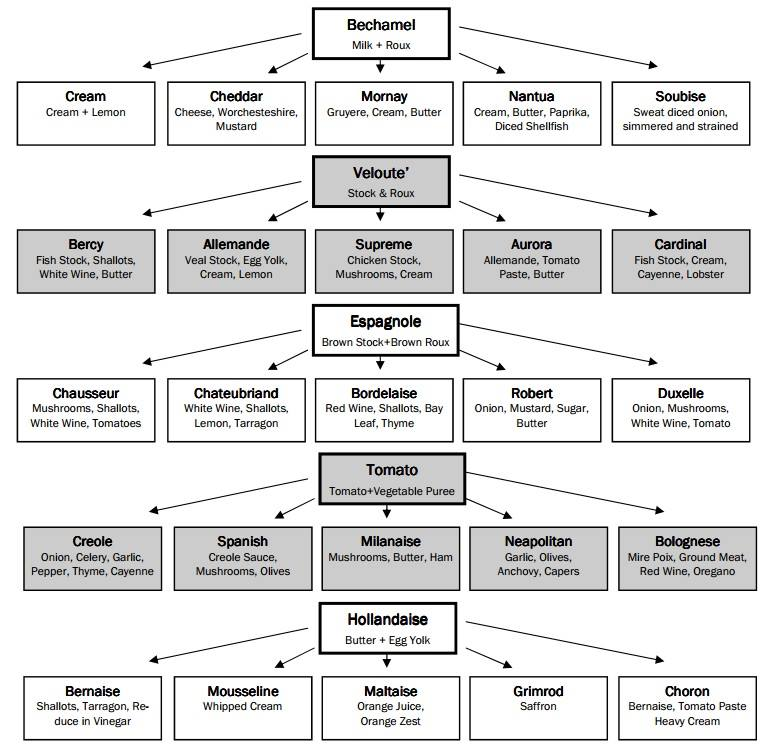
\includegraphics{images/saucer.jpg}
\caption{sovsene}
\end{figure}

Den skal laves til noget egen grafik.

\hypertarget{buxe6rnuxe6se}{%
\section{bærnæse}\label{buxe6rnuxe6se}}

\hypertarget{de-andre-sovse}{%
\section{De andre sovse}\label{de-andre-sovse}}

\hypertarget{steaksovs}{%
\subsection{steaksovs:}\label{steaksovs}}

1/4 cup sennepspulver, Colmans - det er så også den eneste jeg normal kan finde
2 spsk varmt vand
2 spsk risvins eddike - vi prøver nok også med hvidvinseddike
1/4 cup soyasovs

Bland sennepspulver med vandet, og lad det sætte sig et par minutter.

Tilsæt eddike og soyasovs, bland, og passer gennem finmasket si.

Bum. Den skulle blive bedre hvis den får lov at stå på køl mindst en time.

Går også godt med andet - eg fisk.

\hypertarget{cherry-tomat-sovs}{%
\subsection{cherry tomat sovs}\label{cherry-tomat-sovs}}

Fra Noma. Hvor de kalder den for ``Faster than you can boil pasta cherry tomato sauce''

\begin{itemize}
\tightlist
\item
  30 ml oliven olie
\item
  2 fed hvidløg
\item
  200 gram søde cherry tomater
\item
  1½ spsk ``wild rose vinegar''.
\end{itemize}

Skær hvidløgene tyndt, tilføj dem til kold pande, med olivenolien.
Medium varme til de begynder at karamelisere.
Tilsæt de hele tomater, med et generøst drys salt. Låg på.

5-6 minutter senere er tomaterne sprængt og meget bløde. Stavblend til du kan lide konsistensen. Tilføj
eddike (mon ikke vi skal prøve med balsamico), og smag til med mere eddike, salt og peber.

Foldes ind i kogt pasta, og serveres med et drys parmasan ost, et par dråber olie og evt et frisk basilikumblad.

Serveres med 200-300 gram pasta (altså før det koges)

\hypertarget{pebersovs}{%
\subsection{Pebersovs}\label{pebersovs}}

Der skal udvikles yderligere.
Den foreskrev oprindeligt 50 gram peberkorn. Og det var for meget.

2 små skaloteløg
olivenolie
25 gram syltede grønne peberkorn
2 teskeer sennep
7 dl okseboullion
1 sjat whiskey (prøv evt cognac i tstedet)
1 dl fløde
100 gram smør

skalotteløg hakkes og klares i olie.
Peberkorn (knus ca 1/4 af dem med en ske) skylles og tilsættes
sammen med boullion og sennep. Koges ind til ca. det halve.

tilsæt whiskey og fløde - kog et minuts tid ekstra.

Monter med smør, smag til med salt, sukker og peber.

Med 50 gram peberkorn, hvor intet blev mast, skulle der
2 dl fløde til, og den var stadig ret heftig.

\hypertarget{ruxf8get-svampesauce}{%
\subsection{Røget svampesauce}\label{ruxf8get-svampesauce}}

\begin{itemize}
\tightlist
\item
  400 g blandede svampe - skåret i relativt tykke skiver (ca 5 mm)
  *olie
\item
  2 smadrede fed hvidløg
\item
  30 g smør
\item
  45 gram røget svampe garum
\item
  200 gram fløde
\item
  5 gram fint hakkede purløg
\item
  5 gram hakket persille
\item
  salt, peber og citronsaft
\end{itemize}

brun svampene i olien i sauterpande ved middel varme.

tilsæt smør til panden. tilføj hvidløg. rør godt rundt til smørret er smeltet og alt er godt
blandet. ca. 2 minutter.

Steg svampene et par minutter til. Hæld garum i, og steg lidt videre, til
væsken er optaget af svampene. ca. 3 minutter.
tilsæt fløde og lad simre til fløden er reduceret til halvdelen og blevet tykkere.
Tilsæt krydderuerter og smag til med salt, peber og citron.

Også brugbar som pastasovs.

\hypertarget{bistro-sovs}{%
\section{Bistro sovs}\label{bistro-sovs}}

Her er vi i de ægte sovse. En opskrift fra Brødrene

\begin{itemize}
\tightlist
\item
  1 1/4 dl hvidvin
\item
  4 æggeblommer
\item
  1 pakke smør
\item
  1 lille skalotteløg - hakket
\item
  1 bundt purløg - klippet
\item
  1 øko citron
\item
  1 tsk Sennep
\item
  1-2 spsk vineddike. Gerne sherry
\end{itemize}

Eddike, hvidvin og løg koges ind til stort set intet.
Æggeblommer og sennep piskes sammen med essensen. Så piskes det klarede,
lune, smør i ganske som en bærnæse. Smag til med citron, salt og peber.
Principielt bør det nok være hvid peber\ldots{} Men det er vi for dovne til.
Evt også lidt mere eddike.
Rør purløg i, og server.

\hypertarget{portvinssauce}{%
\section{Portvinssauce}\label{portvinssauce}}

\begin{itemize}
\tightlist
\item
  1 gulerod
\item
  1 løg
\item
  1 fed hvidløg
\item
  frisk timian
\item
  1 spsk olie
\item
  2 dl portvin
\item
  2 dl rødvin
\item
  4 dl oksefond
\item
  ½ dl stegesky eller hvad du nu har fra resten af madfremstillingen
\item
  salt, pber, citronsaft og gastrik
\item
  20 gram koldt smør i tern
\end{itemize}

rengør og hak grøntsagerne.
Sauter dem i olien.
Tilsæt portvin, rødvin og hakket frisk timian. Kog ind til det halve.
Hæld oksefonden ved, og kog igen ind til det halve. Tilsæt stegeskyen.
Smag til med salt, peber, citronsaft og gastrik.
Tag sovsen af varmen, sigt den og pisk smørtern i (et ad gangen). Server.

\hypertarget{balsamico-sovs}{%
\subsection{Balsamico sovs}\label{balsamico-sovs}}

\begin{itemize}
\tightlist
\item
  2 spsk rørsukker
\item
  2 spsk balsamico eddike
\item
  1½ dl kalve eller kyllingefond
\item
  2½ dl piskefløde
\item
  Salt, peber, lidt maizenajævner
\end{itemize}

Smelt sukkeret, rør eddiken i. Rør fonden i til sukkeret er opløst. Rør piskefløden i, kog igennem. Juster tykkelsen med lidt maizena, og smag til med salt og peber.

\hypertarget{ostedip}{%
\subsection{Ostedip}\label{ostedip}}

Ikke rigtig en sovs. Men her er den.

\begin{itemize}
\tightlist
\item
  25 g smør
\item
  2 spsk mel
\item
  2 dl mælk
\item
  200 g revet cheddar
\item
  1 fed hvidløg - kvast
\item
  ½ chili eller tørrede chiliflager. Eller bare stødt chili.
\item
  1 tsk NaCl
\item
  1 tsk paprika
\end{itemize}

Smelt smørret med krydderier, salt og hvidløg

Bag op med mel og mælk.

Tilsæt osten og varm op til den er helt smeltet.

Smag til, og nej, der skal nok ikke mere salt i!

Juster tykkelsen med mælk, og server så snart den er færdig. Ellers serverer du ikke en dip, men en klods.

\hypertarget{kondimenterne}{%
\chapter{kondimenterne}\label{kondimenterne}}

\hypertarget{syltede-champignon}{%
\section{Syltede champignon}\label{syltede-champignon}}

\begin{itemize}
\tightlist
\item
  500 gram hvide champignons, rensede og rodskårne
\item
  2 dl mørk balsamico
\item
  2 dl olivenolie
\item
  1 spsk salt
\item
  20 sorte peberkorn
\item
  5-8 laurbærblade
\end{itemize}

Rør alt andet end svampene sammen - grundigt
Læg svampe i sterilt glas, hæld lage over, og lad trække i
to døgn. Spises som tilbehør til grillet kød, som tapas elleer
i salater

\hypertarget{trykkogerketchup}{%
\section{Trykkogerketchup}\label{trykkogerketchup}}

efter www.hippressurecooking.com/pressure-cooker-ketchup-recipe
og Dansk Kemi 2020 (6) p.~38 - 39, ved Jens Folke

\begin{itemize}
\tightlist
\item
  1 kg blommetomater skåret i kvarte
\item
  15 g paprika
\item
  5 g salt
\item
  1 g stødt kanel
\item
  1 g nelliker stødt
\item
  2 g hvidløgspulver
\item
  2 g sellerifrø
\item
  10 g dijonsennep
\item
  15 g honning
\item
  80 g rosiner
\item
  1/4 zittauerløg
\item
  85 ml æbleeddikke
\item
  15 g majsstivelse rørt ud i 15 ml vand
\end{itemize}

Kan yderligere krydres med chili, røget paprika, æble, korianderfrø
m.m.m

Smid alt undtagen majsstivelse og vand i trykkogeren.

Mos tomaterne nok til at væsken når op på trykkogerens minimumsbehov
bring trykkogeren under tryk, når den når 2 atmosfærer, lad koge i
5 minutter
Tag trykket af, og lad det koge ind i 10 minutter - reduceres til knap
halvdelen.

Bland majsstivelse i vand, og hæld det i - lad det koge med.

Smadr blandingen med stavblender - passer gennem sigte.

\hypertarget{skalottemarmelade}{%
\section{Skalottemarmelade}\label{skalottemarmelade}}

giver 1½ kop

\begin{itemize}
\tightlist
\item
  Neutral olie
\item
  1 kg skalotter - pillet og hakket
\item
  3/4 teske salt
\item
  ½ kop sukker
\item
  6 spiseskeer malteddike - eller anden eddike.
\end{itemize}

Olie i sauterpande.
Løg og salt i pande.
``kog'' under låg i ca. ti minutter. Rør undervejs, til løgene er klare
skru ned for varmen og tag låget af.
tilsæt sukker og 1 spsk vand. simrer i 30 minutter. deglacer med 1 spsk vand efter behov.
rør derefter fire spsk eddike i. simrer videre i 10-15 minutter, til konsistensen er jammy.
rør den resterende eddike ind, og sluk for varmen.
Smag til.
Hæld på glas (skoldet etc)

\hypertarget{fars-nylon}{%
\section{Fars nylon}\label{fars-nylon}}

Aka 1000 øers dressing

\begin{itemize}
\tightlist
\item
  Mayo - svarende til af en æggeblomme og 3 dl olie
\item
  1 spsk creme fraiche
\item
  1 spsk tomatpure
\item
  1 tsk engelsk sovs
\item
  1 knivsspids paprika
\item
  1 smule tabasco
\item
  1 smule cognac
\item
  1 smule sukker
\end{itemize}

Det hele blandes sammen.

\hypertarget{worcestershire-sauce---engelsk-sovs}{%
\section{Worcestershire Sauce - Engelsk sovs}\label{worcestershire-sauce---engelsk-sovs}}

Eller hvad pokker det nu hedder\ldots{}

500 ml Æble eddike
4 fed hvidløg
120 g skalotteløg
30 g ansjosfilleter
60 g honning
60 g rørsukker eller melasse
60 g tamarind paste
2 tsk chilipulver
1 tsk stødte nelliker

Alt smides i en gryde, og der stavblendes til det er så smooth som muligt.

varm op ved medium varme til den koger. Skrug ned til lav varme og lad simre
i 15 minutter under omrøring.

Herfra er der to metoder:

\begin{enumerate}
\def\labelenumi{\arabic{enumi}.}
\tightlist
\item
  Filtrer gennem kaffefilter. Lad det dræne en times tid. Rør let i pastaen
  så det meste kommer igennem. (brug evt først det fine nylonfilter).
\end{enumerate}

Tilsæt tre tsk af filterkagen til filtratet, ryst grundigt og hæld straks på
rengjorte skoldede (evt atamonskyllede) flasker. Opbevar mørkt og køligt
(men ikke i køleskabet). Lad den lagre mindst 2 måneder, helst 18 måneder.

Filterkagen kan med fordel gemmes og tilsættes supper, gryderetter eller andet godt.

\begin{enumerate}
\def\labelenumi{\arabic{enumi}.}
\setcounter{enumi}{1}
\tightlist
\item
  Hæld sovsen direkte på rengjorte, skoldede, evt. atamonskyllede flasker.
  Den lagres ligeså længe. Der er frit valg ang. filtrering efter den har lagret.
\end{enumerate}

\hypertarget{specialiteterne}{%
\chapter{Specialiteterne}\label{specialiteterne}}

\hypertarget{konfiterede-hvidluxf8g}{%
\section{Konfiterede hvidløg}\label{konfiterede-hvidluxf8g}}

Et lille sylteglas fyldes med pillede hvidløg

Salt kommes i (hvor meget?) sammen med krydderier.

rosmarin og rosenpeber skulle være godt.

Så fyldes glasset med en god olie og låget lukkes til.

Sous vides det i 3-4 timer på 87 grader

\hypertarget{saltede-uxe6ggeblommer}{%
\section{Saltede æggeblommer}\label{saltede-uxe6ggeblommer}}

Fyld et par centimeter fint (IKKE groft) salt i en bøtte.
Skil blommer fra æg, og placer dem på saltet. Dæk fuldsændigt med salt
Lad stå i køleskabet 8 timer.
Pil æggeblommerne op af saltet, skyl dem i koldt vand, tør dem. Og
tør dem i ovnen vad 60 grader - 2 timer er for lidt, opskriften sagde også 3.
De er for gummiagtige, så de skal have længere end det.

Målet er at de skal kunne rives. Så de skal være ret hårde og tørre.

\hypertarget{sous-vide-kold-kaffe}{%
\section{sous vide kold kaffe}\label{sous-vide-kold-kaffe}}

½ cup (så volumen mål) groft kværnet kaffe
4 cup vand

kaffe og vand i vandtæt syltetøjsglas. Sousvides i 2-4 timer ved 150 grader F.

Filtrer, og server hældt over is, eller opbevar på køl i en uges tid.
Overvej om den skal fortyndes.

\hypertarget{rester}{%
\chapter{Rester}\label{rester}}

Vi skal af med resterne

\hypertarget{standardmuxe5der}{%
\section{Standardmåder}\label{standardmuxe5der}}

\begin{itemize}
\tightlist
\item
  Standard pastabix - Se under pastaretterne
\item
  Bixemad
\end{itemize}

\hypertarget{gratin}{%
\section{Gratin}\label{gratin}}

Dette er basisopskriften. Den skal bruges til at skaffe os af med rester.

\begin{itemize}
\tightlist
\item
  100 g smør
\item
  150 g mel
\item
  3 dl grøntsagsbouillon
\item
  3 dl sødmælk
\item
  8 æg
\item
  salt, peber, rasp
\end{itemize}

mindst 50 gram rester, men den kan sagtens trække en del mere.
Skær resterne i mindre stykker

Smelt smør, rør sammen med mel. Lav grundlæggende en opbagt
sovs med væsken.
Del æggene, tag gryden af varmen, og rør blommerne i,.

Pisk hviderne stive, vend halvdelen i gryden sammen med fyldet.

Vend resten af hviderne i. Smør et fad/skål
og drys med rasp. drys rasp over gratinen, bag nederst i ovnen
ved 175 grader i ca. 1 time. Server med smeltet smør.

\hypertarget{hapsere-tapas-med-videre.}{%
\chapter{Hapsere, tapas med videre.}\label{hapsere-tapas-med-videre.}}

\begin{Shaded}
\begin{Highlighting}[]
\FunctionTok{library}\NormalTok{(ggplot2)}
\NormalTok{generate\_circle }\OtherTok{\textless{}{-}} \ControlFlowTok{function}\NormalTok{(}\AttributeTok{center =} \FunctionTok{c}\NormalTok{(}\DecValTok{0}\NormalTok{, }\DecValTok{0}\NormalTok{), }\AttributeTok{radius =} \DecValTok{1}\NormalTok{, }\AttributeTok{n\_points =} \DecValTok{100}\NormalTok{) \{}
\NormalTok{  theta }\OtherTok{\textless{}{-}} \FunctionTok{seq}\NormalTok{(}\DecValTok{0}\NormalTok{, }\DecValTok{2} \SpecialCharTok{*}\NormalTok{ pi, }\AttributeTok{length.out =}\NormalTok{ n\_points)}
  \FunctionTok{data.frame}\NormalTok{(}
    \AttributeTok{x =}\NormalTok{ center[}\DecValTok{1}\NormalTok{] }\SpecialCharTok{+}\NormalTok{ radius }\SpecialCharTok{*} \FunctionTok{cos}\NormalTok{(theta),}
    \AttributeTok{y =}\NormalTok{ center[}\DecValTok{2}\NormalTok{] }\SpecialCharTok{+}\NormalTok{ radius }\SpecialCharTok{*} \FunctionTok{sin}\NormalTok{(theta)}
\NormalTok{  )}
\NormalTok{\}}
\NormalTok{circle\_data }\OtherTok{\textless{}{-}} \FunctionTok{generate\_circle}\NormalTok{(}\AttributeTok{center =} \FunctionTok{c}\NormalTok{(}\DecValTok{0}\NormalTok{, }\DecValTok{0}\NormalTok{), }\AttributeTok{radius =} \DecValTok{1}\NormalTok{)}

\CommentTok{\# Generer data til linjerne}
\NormalTok{generate\_lines }\OtherTok{\textless{}{-}} \ControlFlowTok{function}\NormalTok{(}\AttributeTok{center =} \FunctionTok{c}\NormalTok{(}\DecValTok{0}\NormalTok{, }\DecValTok{0}\NormalTok{), }\AttributeTok{radius =} \FloatTok{1.5}\NormalTok{) \{}
\NormalTok{  angles }\OtherTok{\textless{}{-}} \FunctionTok{seq}\NormalTok{(}\DecValTok{0}\NormalTok{, }\DecValTok{2} \SpecialCharTok{*}\NormalTok{ pi, }\AttributeTok{length.out =} \DecValTok{9}\NormalTok{)[}\SpecialCharTok{{-}}\DecValTok{9}\NormalTok{] }\CommentTok{\# Otte vinkler (0, π/4, π/2, ..., 7π/4)}
  \FunctionTok{data.frame}\NormalTok{(}
    \AttributeTok{x =} \FunctionTok{rep}\NormalTok{(center[}\DecValTok{1}\NormalTok{], }\AttributeTok{each =} \FunctionTok{length}\NormalTok{(angles)),}
    \AttributeTok{y =} \FunctionTok{rep}\NormalTok{(center[}\DecValTok{2}\NormalTok{], }\AttributeTok{each =} \FunctionTok{length}\NormalTok{(angles)),}
    \AttributeTok{xend =}\NormalTok{ center[}\DecValTok{1}\NormalTok{] }\SpecialCharTok{+}\NormalTok{ radius }\SpecialCharTok{*} \FunctionTok{cos}\NormalTok{(angles),}
    \AttributeTok{yend =}\NormalTok{ center[}\DecValTok{2}\NormalTok{] }\SpecialCharTok{+}\NormalTok{ radius }\SpecialCharTok{*} \FunctionTok{sin}\NormalTok{(angles)}
\NormalTok{  )}
\NormalTok{\}}
\NormalTok{line\_data }\OtherTok{\textless{}{-}} \FunctionTok{generate\_lines}\NormalTok{(}\AttributeTok{center =} \FunctionTok{c}\NormalTok{(}\DecValTok{0}\NormalTok{, }\DecValTok{0}\NormalTok{), }\AttributeTok{radius =} \DecValTok{1}\NormalTok{)}


\FunctionTok{ggplot}\NormalTok{() }\SpecialCharTok{+}
  \FunctionTok{geom\_path}\NormalTok{(}\AttributeTok{data =}\NormalTok{ circle\_data, }\FunctionTok{aes}\NormalTok{(}\AttributeTok{x =}\NormalTok{ x, }\AttributeTok{y =}\NormalTok{ y), }\AttributeTok{size =} \DecValTok{1}\NormalTok{) }\SpecialCharTok{+}
  \FunctionTok{geom\_segment}\NormalTok{(}\AttributeTok{data =}\NormalTok{ line\_data, }\FunctionTok{aes}\NormalTok{(}\AttributeTok{x =}\NormalTok{ x, }\AttributeTok{y =}\NormalTok{ y, }\AttributeTok{xend =}\NormalTok{ xend, }\AttributeTok{yend =}\NormalTok{ yend), }\AttributeTok{linetype =} \StringTok{"dashed"}\NormalTok{) }\SpecialCharTok{+}
  \FunctionTok{coord\_equal}\NormalTok{() }\SpecialCharTok{+}
  \FunctionTok{theme\_minimal}\NormalTok{()}
\end{Highlighting}
\end{Shaded}

\begin{verbatim}
## Warning: Using `size` aesthetic for lines was deprecated in ggplot2 3.4.0.
## i Please use `linewidth` instead.
## This warning is displayed once every 8 hours.
## Call `lifecycle::last_lifecycle_warnings()` to see where this warning was
## generated.
\end{verbatim}

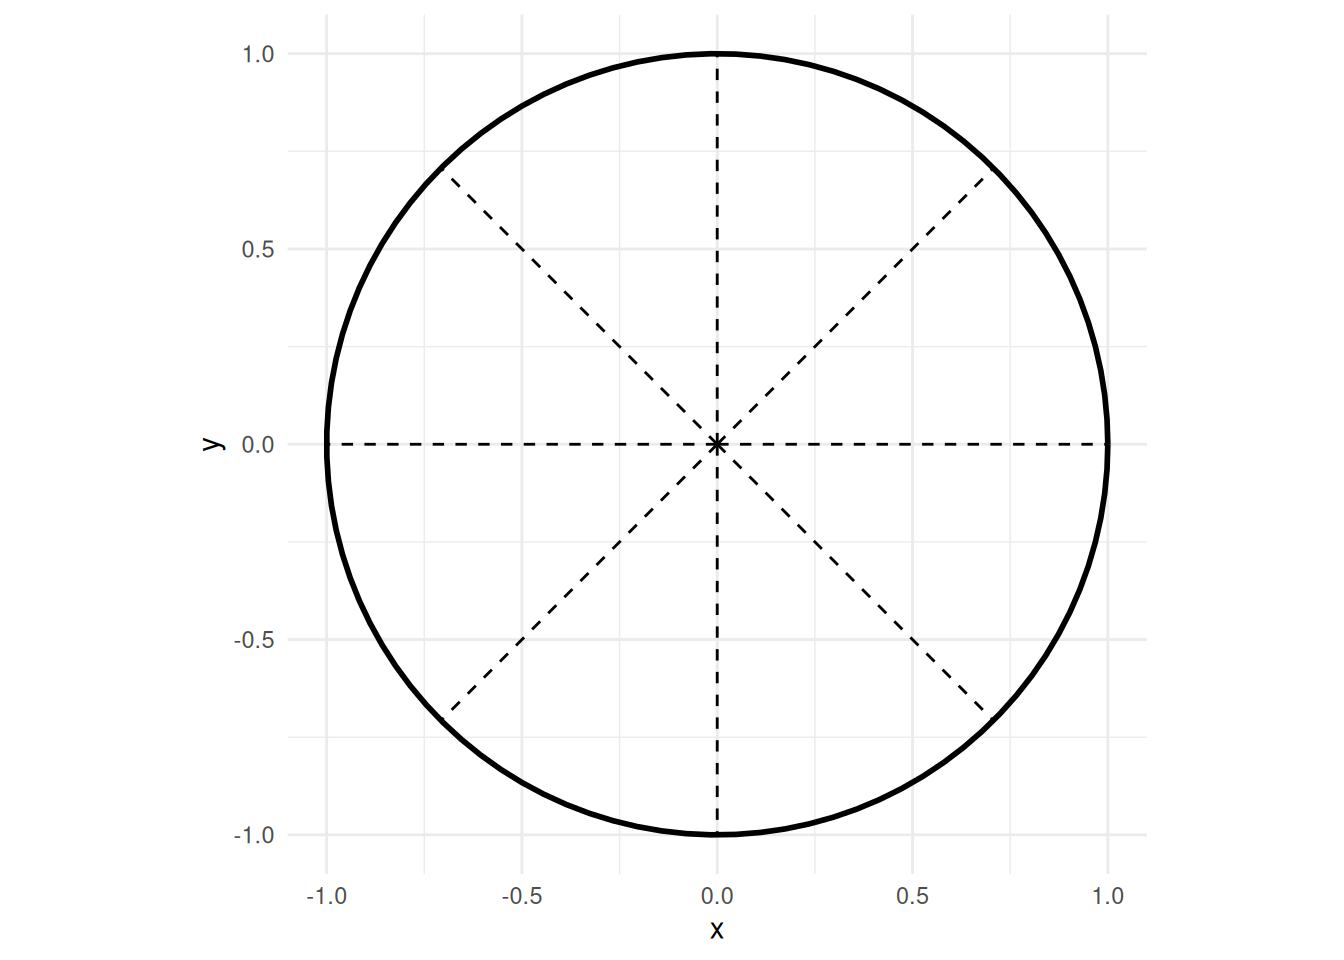
\includegraphics{Kogebog_files/figure-latex/unnamed-chunk-1-2.pdf}

\hypertarget{toskanske-buxf8nner}{%
\section{Toskanske bønner}\label{toskanske-buxf8nner}}

Jeg har aldrig forstået hvorfor de der hvide bønner skulle kunne bruges til
andet end at kaste efter folk.

Indtil vi fik en anretning på en restaurant i Firenze vi havde fundet i en
reklametryksag fra et dækfirma.

Fagioli all'uccelletto

\begin{itemize}
\tightlist
\item
  600 gram hvide bønner (helt oprindeligt - cannellini)
\item
  olivenolie
\item
  lidt salvie blade
\item
  to fed hvidløg
\item
  2 spsk tomat pure
\item
  4 ferske svinepølser (og her dur det altså ikke med grillpølser\ldots)
\item
  salt og peber
\end{itemize}

Bønnerne skal ligge i blød. Og så skal de koges. Gerne i noget bouillon.

Så varmer vi et par spiseskeer olie op på en pande med hvidløget -
bare lad skindet være på dem, og knus dem med hånden - og salvien

Når olien har taget smag af hvidløget, og salvien er blevet sprød,
hælder vi bønnerne op i panden, sammen med en god sjat af deres kogevand.
Tilføjer tomatpastaen, rører rundt og koger ved lav temperatur. Lad dem
simre i 20 minutter, pil pølserne ud af deres skind, og smid dem i. Lad det yderligere
simre til pølserne er færdige. Server med brød.
\url{https://www.visittuscany.com/en/recipes/fagioli-alluccelletto-tuscan-style-beans-recipe/1111}

\hypertarget{gougeres}{%
\section{Gougeres}\label{gougeres}}

Giver to fulde bageplader!
100 g hvedemel
90 g smør
1 dl vand
1 dl sødmælk
1⁄2 tsk. groft salt
1⁄2 tsk. sukker
3 store æg L/XL, sammenpiskede (ca. 180 g)
100 g revet gruyère ELLER 150 g frisk gedeost samt kværnet sort peber
1. Forvarm ovnen til 200° uden varmluft. Beklæd to bageplader med bagepapir.
2. Sigt melet -- gerne ned på et stykke bagepapir, da det så kan hældes hurtigt i gryden.
3. Smelt smørret sammen med vand, mælk, salt og sukker i en gryde ved moderat varme. Når smørret er
smeltet, bringes det hele i kog ved høj varme og tages straks af varmen. Hæld det sigtede mel i gryden,
og rør med en træske, indtil det bliver til en fast, blød dej uden klumper, der slipper gryden.
4. Sæt gryden tilbage på kogepladen på svag varme for at 'riste' dejen i et par minutter. Rør forsigtigt i
dejen mens den ristes, og undlad at skrabe i bunden af gryden. Der vil sætte sig et meget tyndt lag dej,
som ikke skal blandes sammen med resten af dejen igen.
5. Hæld dejen i en skål, og lad den køle lidt af (i ca. 5 minutter). Hvis du bruger røremaskine, kan du
med fordel hælde dejen i røreskålen og lade den køre rundt med 'det flade piskeris' på lav til
mellemhastighed. På den måde køles dejen hurtigt.
6. Tilsæt de sammenpiskede æg ad tre omgange, og rør energisk efter gang for at få massen homogen.
På røremaskine røres fortsat med lav til mellemhastighed med det flade piskeris. Når æggene tilsættes,
vil dejen først se ud som om den skiller, men vil samle sig igen efter omrøring.

\begin{enumerate}
\def\labelenumi{\arabic{enumi}.}
\setcounter{enumi}{6}
\tightlist
\item
  Fortsæt med at røre i dejen i nogle minutter, så den bliver godt elastisk. Dejen er klar når den er glat
  og skinnende.
\item
  Tilsæt revet gruyère eller snuldret gedeost (samt evt. peber eller krydderurter).
\item
  Overfør dejen til bagepladen med sprøjtepose, skeer eller en isske. Sæt små klatter på størrelse med
  en femmer til hors d'oeuvre eller store, hvis de skal spises som mellemmåltid.
\item
  Lav et kryds (gittermønster) på toppen af hver gougère med en gaffel dyppet i vand, så hæver de
  flottere i ovnen.
\item
  Sæt bagepladen i den varme ovn, og skru så ned til 170°. Lad dem bage i mindst 20 minutter uden at
  åbne ovndøren. Bagetiden afhænger af størrelsen. De er færdige, når de er jævnt lysebrune. De må
  gerne bages lidt mindre end vandbakkelser, som skal fyldes med creme. De er nemlig lækrest, hvis de er
  svampede indeni.
  TIP: Sæt gerne en ekstra bageplade i ovnen under pladen med vandbakkelser, så de ikke bliver brændte
  i bunden.
\end{enumerate}

\hypertarget{hummus}{%
\section{Hummus}\label{hummus}}

En dåse kikærter (vægt drænet?)
En toppet spiseskefuld tahin
Citronsaft
1 tsk spidskommen
½ dl koldt vand
en isterning
3 spsk olie
salt og peber

\hypertarget{bagt-camenbert}{%
\section{Bagt camenbert}\label{bagt-camenbert}}

I airfryer. Et stk camembert. Ikke en af de helt store - ikke en af de helt små.

Skær tern i overfladen af osten, en centimeters penge på hver led.
Pensl med trøffelolie, hakket frisk timian, honning og chili. Noget mere end man
lige tror.

Bag i airfryeren ved 160 grader i 12 minutter. Lækkert.

\hypertarget{cheeseburger-buket}{%
\section{Cheeseburger buket}\label{cheeseburger-buket}}

tortillas smøres med hakket kød, og skæres i halve.
En trekant cheddarskive lægges på (bred side mod rundingen i tortillaen.
Tortillaen rulles til et kræmmerhus, og placeres i en rundform. 12 stykker eller
deromkring. i ovnen til kødet er tilberedt. Rdys med hakkede rødløg, hakkede
cornichoner og server med ostesovs.

Jeg er skeptisk overfor det med det rå kød. Så jeg steger det først\ldots{}
ud mod rundingen af )

\hypertarget{desserterne}{%
\chapter{Desserterne}\label{desserterne}}

\hypertarget{salt-og-peber-is}{%
\section{Salt og peber is}\label{salt-og-peber-is}}

454 gram piskefløde
1 spsk sorte peberkorn
½ tsk sorte peberkorn
150 gram sukker
1 spsk vodka
½ tsk salt
flage salt

knus 1 spsk peberkorn groft i en morter.
varm fløden op til den damper. tag af varmen, og rør de
knuste peberkorn i. Lad det trække en time - rør regelmæsigt.
Knus ½ tsk peber fint.

Sig fløden og smid peberkornene ud. Tilføj sukker,
vodka og salt, og rør indtil sukkeret er opløst.
Rør det fintmalede peber i. Dæk og køl til meget
koldt, mindst et par timer, op til en dag.

Pisk flødeskummen til meget bløde toppe.

Frys 8 - 12 timer.

Smid lidt flagesalt på toppen.

Hertil kan serveres en salt og peber brittle.

1 tsk sorte peberkorn
½ kop (99 gram) sukker
flagesalt.

Mal peberen - vi skal have et mix af groft og fint.
Dæk bageplade med bagepapir.
Smid sukkeret i en lille kaserolle, og giv den 3
spsk vand. Bring i kog over middel varme,
og kog til det har samme farve som mørk ahornsirup.
Undgå at røre, swirl kaserollen i stedet.
Så snart karameliseringen er sket - tages den af varmen, og der røres (silikoneredskaber er din ven her) stødt peber . Over på bagepapiret - spred ud så tyndt som muligt, så hurtigt som jmuligt. Og spred
flagesalt over med det samme!

Lad det køle helt ned - mindst 15 minutter, knus til mindre stykker - og opbevar i luftæt beholder.

\hypertarget{bagning}{%
\chapter{Bagning}\label{bagning}}

\hypertarget{koldhuxe6vede-morgenboller}{%
\section{Koldhævede morgenboller}\label{koldhuxe6vede-morgenboller}}

Goto opskriften, fordi den kan røres sammen aftenen i forvejen.

\begin{itemize}
\tightlist
\item
  6 dl vand
\item
  25 g gær
\item
  15 gram akaciehonning
\item
  480 gram hvedemel
\item
  65 gram solsikkekerner
\item
  270 gram durummel
\item
  2 tsk salt
\end{itemize}

Rør gæren ud i vandet.
Rør honningen ud i gærblandingen

Bland kerner og hvedemel.

Bland salt og durummel (tipo 00 fungerer også fint).

Rør durummel i gærblandingen.
Rør hvedemel i dejen.

Rør sammen til dejen er jævn, klæg, og har en skinnende/våd
overflade

Hæver tildækket to timer på køkkenbordet, eller natten over
på køl.

Forvarm ovnen til 225 grader varmluft. Sæt bollerne på to
plader, 8 på hver. Gør det med våde hænder.

Bages ca. 17 minutter, til de har en let gylden overflade.

Dette er en god basis opskrift. Der kan hældes flere/færre/andre
kerner i. Eller der kan tilsættes havregryn eller grovere
mel i - i så fald skal der formentlig lidt mere væske i, da
havregryn eller groft mel suger mere væske.

\hypertarget{fuglebruxf8d}{%
\section{fuglebrød}\label{fuglebruxf8d}}

Almindelig brøddej. Og så formet på denne måde:
\includegraphics{images/fuglebrød.jpg}
Gerne en lille rosin eller korender som øje.

\hypertarget{preservationerne}{%
\chapter{Preservationerne}\label{preservationerne}}

\hypertarget{uxe6blesmuxf8r}{%
\section{Æblesmør}\label{uxe6blesmuxf8r}}

\begin{itemize}
\tightlist
\item
  2487 gram æbler, skrællet, og kernehus fjernet
\item
  1,2 l vand
\item
  3 stjerneanis
\item
  vanillestang - eller vanillesukker
\item
  3 kanelstænger
\end{itemize}

Koges til mos.

Mosen paseres gennem sigte - vi skal af med stjerneanisen.
Det er hård arbejde, så sæt god tid af.

Mosen over i en ren gryde/sauterpande eller lignende.
Kog sammen vanillestangen (eller sukkeret), samt kanelstængerne.
Simrer roligt under låg 1½ til 2 timer, til det bliver mørkt og tykt.

\hypertarget{diverse-og-usorteret}{%
\chapter{Diverse og usorteret}\label{diverse-og-usorteret}}

\hypertarget{den-faste-madplansrotation}{%
\section{den faste madplansrotation}\label{den-faste-madplansrotation}}

\hypertarget{kartoffelfrikadeller}{%
\section{kartoffelfrikadeller}\label{kartoffelfrikadeller}}

500 gram kartoffelmos
1 revet løg
1 æg
3-4 spsk hvedemel
4-5 spsk rasp
salt og peber

Rør alt sammen, steg dem 2-3 minutter i olie/smør

Nappet fra Maden i mit liv siden.

\url{https://gastrofun.dk/opskrift/koral-tuille/}

Bechamel - Mælk + roux
bliver til
Cream (cream + lemon)
Cheddar (chees, worchestershire sovs, mustard

\hypertarget{svampe-omelet}{%
\section{Svampe omelet}\label{svampe-omelet}}

Også fra Noma

\begin{itemize}
\tightlist
\item
  20 gram røget svampe garum
\item
  100 g assorterede svampe - tyndt skåret
\item
  olie
\item
  30 gram smør
\item
  1 fed hvidløg - smadret
\item
  5 gram purløg - hakket
\item
  2 store æg
\item
  salt og peber
\end{itemize}

brun svampene i olien i en sauterpande.

tilsæt halvdelen af smøret, og de knuste hvidløg
toss svampene, så de dækkes af hvidløgssmør.
Lad dem stege videre et par minutter, hæld svampe garum over. Steg videre til væsken er reduceret lidt.

Tilføj purløg, og bland. Overfør til skål.

Pisk æggene.

Hold hånden over en pande 3 cm. i to sekunder. Hvis det er for varmt, skru ned, hvis ikke, skru op.
hæld den anden halvdel af smørreet påå panden og fordel.
Hæld æg på panden. de skal boble roligt. fordel over hele panden. agiter æggene med en paletkniv.
Toppen skal være løs og creamy. Salt æggene.

fjern panden fra varmen, o hæld svampene ud på midten af omeletten.
Fold omeletten over sig selv, så svampene dækkes. Vi går efter en halvmåne form.

Løft omeletten, og snig en smule smør ind under den. Giv den varme i ca. 30 sekunder. Server.

\hypertarget{bagselv-leverpostej-i-airfryer}{%
\section{bagselv leverpostej i airfryer}\label{bagselv-leverpostej-i-airfryer}}

Det forlyder - men er ej testet, at den bages direkte fra
frost ved 170 grader i 40 minutter.
Det tester vi så!

\hypertarget{lidt-mere-teoretisk}{%
\chapter{Lidt mere teoretisk}\label{lidt-mere-teoretisk}}

\hypertarget{svampe}{%
\section{Svampe}\label{svampe}}

Noget af det magiske ved svampe er deres indhold af frie aminosyrer. Især
glutaminsyre. Når den nedbrydes under tilberedningen, får vi på helt naturlig
vis mononatriumglutamat, eller det utroligt farlige MSG som veganere og andre
med forkærlighed for svampe er meget bange for. Nej, jeg forstår heller ikke
logikken.

Anyway, MSG fra svampe er koncentreret umami, særlig mundfylde - og så forstærker
det ca. alle andre smage.

Det viser sig i forskningen at glutamats smag mere end fordobles, hvis det kombineres
med visse nukleinsyrer - og netop tørrede svampe har en høj koncentration af
nukleinsyren guanylat. Og så er der fuld skrue på umamismagen.

Svampe er ikke grøntsager:


\includegraphics{images/svampe.png}

Men de har især særligt stærke cellevægge. De indeholder kitin, der ikke er
vandopløseligt, i modsætning til planters cellevægge, der bruger pektin i samme
rolle.

Det betyder at svampene bevarer (mere) af deres struktur ved tilberedning. Det
er endnu en af årsagerne til at de minder en del om kød i både smag og tekstur.

Store dele af forskellene mellem de forskellige spisesvampe er knyttet til duftstofferne.
Octenol giver noter af skovbund, men noterne spænder fra mandler til skaldyr.

For de fleste svampe gælder det at deres aromastoffer intensiveres når de tørres.

En frisk svamp indeholder ca 80\% vand. Det skal reduceres ved tilberedningen, og
det gøres bedst ved moderat varme i længere tid, gerne tørstegning, så vandet
fordamper letere. Når vandet er delvist fordampet, har vi fået aktiveret
aminosyrer, nukleinsyrer og aromastoffer kemisk. Og så skruer vi op for varmen.
Det er her vi tilsætter fedtstof - af god smag og kvalitet, da svampene optager
det og tager smag af det.

Møre svampe giver generet mest smag og duft. Bortset fra trøfler. Den hvide dufter
mest, den sorte sommertrøffel er kraftigst i smagen.

De mørkere svampe der i tørret udgave giver mest umami, er Karl Johan, morkler,
shitake og matsutake. Og eftersom friske stegte svampe optager smagen af det
de bliver stegt med, kan man få helt almindelige champignoner til at smage af
meget mere, hvis man steger dem med udblødte tørrede karljohaner.

Det er duftstofferne der bidrager mest - og derfor handler det om at fastholde
dem så godt som muligt. Mange af duftstofferne kan kun registreres gennem næsen,
men ikke ad mundhulen når vi tygger svampen. Derfor kan trøfler virke skuffende,
hvsi vi ikke binder nogen af de flygtige stoffer i fedt.

Da trøfler ikke særligt godt tåler varme, gøres det bedst i form af spejlæg eller
pasta med smør - som vi så høvler trøfler over i stedet for at give dem varme.

De fleste andre svampe har helt generelt bedst af at blive varmebehandlet og
få et skud godt fedst for at fastholde duftstofferne. Det gælder både morkler,
men også kantareller.

Så - kombiner de sjældnere vilde svampe, med de mildere dyrkede svampe,
der tager smag af de vilde - og giver fylde og struktur i retten.

\hypertarget{omregninger-og-muxe6ngder}{%
\chapter{omregninger og mængder}\label{omregninger-og-muxe6ngder}}

Ved kogning af pasta er reglen:

1000/100/10. Som i 1000 g vand, 100 g pasta og 10 g NaCl

\hypertarget{us--til-civiliserede-muxe5l}{%
\section{US- til civiliserede mål}\label{us--til-civiliserede-muxe5l}}

\begin{itemize}
\tightlist
\item
  1 oz \textasciitilde{} 28 gram
\item
  375 F \textasciitilde{} 190 grader C
\item
  1 cup = 273 ml
\item
  1 pint = 2 cups = 546 ml
\end{itemize}

\hypertarget{volumenvuxe6gt}{%
\section{Volumen/vægt}\label{volumenvuxe6gt}}

\hypertarget{generelt}{%
\subsection{Generelt}\label{generelt}}

\begin{itemize}
\tightlist
\item
  1 spsk = 15 ml
\item
  1 tsk = 5 ml
\end{itemize}

\hypertarget{specifikke}{%
\subsection{Specifikke}\label{specifikke}}

\begin{itemize}
\tightlist
\item
  1 spsk groft salt = 22 gram
\item
  1 tsk groft salt = 7 gram
\end{itemize}

\hypertarget{muxe6ngder}{%
\section{Mængder}\label{muxe6ngder}}

\hypertarget{pastasalat-til-madpakke}{%
\subsection{pastasalat til madpakke}\label{pastasalat-til-madpakke}}

Vi skal have mængderne på plads her!

300 gram tør discount fusili vejer
681 gram kogt.

Så skal vi have styr på hvor meget der skal til for at gøre det ud for frokost. Og så
finde ud af hvor meget det fylder - så beholder størrelse kan justeres.

Testet 21. januar.

2229 gram pastasalt, inklusive den hvide margretheskål.

Så spiste vi begge to - vi fik nok. Og skålen, inklusive
resten af salaten vejede 1359 gram

Resten af pastasalaten vejede - uden emballage 625 gram.

Salaten blev lavet af ovenstående 681 gram pasta, 240 gram
majs, 200 gram salattern og 250 gram tomater. Hertil rigelige
mængder thousand island dressing

Vi fik med andre ord 870 gram pastasalat i alt, eller 435 gram hver.

Og ialt blev der produceret
2229-1359 = 870, det vi spiste.
+ 625 gram, det der var til rest.
Så i grove træk får vi 1495 gram pastasalat af at koge 300 gram
tør pasta. Hvis vi regner med 500 gram færdig pastasalt,
går der derfor 100 gram tør pasta til en frokostportion pastasalat

Vi kan yderligere notere, at et 3/4 liters fido sylteglas med
patentlukning, uden de store problemer holder ca. 500 gram
pastasalat. Det er nu min madpakkebeholder!

\end{document}
